\begin{figure}

\centering

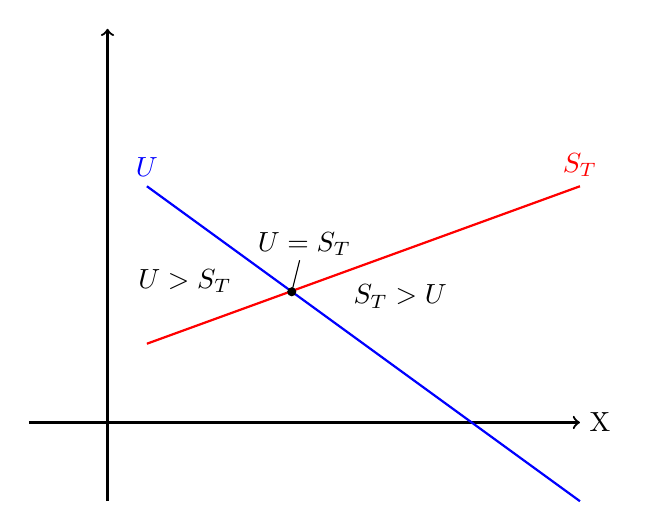
\begin{tikzpicture}

% Axes
\draw [->, thick] ( -1, 0 ) -- ++( 7, 0 );
\draw [->, thick] ( 0, -1 ) -- ++( 0, 6 );

% U profile
\draw [blue, thick] ( 0.5, 3 ) -- ++( 5.5, -4 );

% S_T profile
\draw [red, thick] ( 0.5, 1 ) -- ++( 5.5, 2 );

% Flame stabilization location
\filldraw ( 2.34, 1.66 ) circle ( 0.05 ) -- ++( 0.1, 0.4 );

% Labels
\node at ( 6, 0 ) [right] {X};
\node at ( 0.5, 3 ) [above,blue] {\(U\)};
\node at ( 6, 3 ) [above, red] {\(S_T\)};

\node at ( 2.5, 2 ) [above] {\(U=S_T\)};
\node at ( 1.7, 1.8 ) [left] {\(U>S_T\)};
\node at ( 3, 1.6 ) [right] {\(S_T>U\)};

\end{tikzpicture}

\caption[Schematic of LSB flame stabilization]{The figure above illustrates the robustness of the LSB flame stabilization mechanism. The flame is stabilized at the point where the reactant velocity, \(U\), and the turbulent flame speed, \(S_T\), are equal. Perturbations to the flame standoff distance to the left or the right are counteracted by either \(U\) or \(S_T\) respectively making this a stable equilibrium.}

\label{fig:flameEquilibrium}

\end{figure}

